% This is document is based on the samplepaper.tex, a sample chapter demonstrating the LLNCS macro package for Springer Computer Science proceedings;
% Version 2.20 of 2017/10/04
%
\documentclass[runningheads]{llncs}
\usepackage{graphicx}
%
\begin{document}
%
\title{GDPR's Issue: Not Cost But Forced Consent}
% 
\author{Quentin Le Roux\inst{1}}
%
\institute{Université Côte d'Azur \email{quentin.leroux@edhec.fr}}
%
\maketitle
%
\begin{abstract}
This paper presents a short summary of the aims outlined in the European General Data Protection Regulation (GDPR) corpus of laws and highlights the main shortcoming that has emerged since its inception: Not the early concerns about competition and business impacts, but rather how the rise of dark patterns has shown that the issue of informed consent is not solved yet.
%
\keywords{GDPR \and informed consent \and dark patterns.}
\end{abstract}
%
\section{Introduction}
Implemented in 2018 with \textit{fanfare}, GDPR was supposed to be a nail in the coffin of an ineffective Data Protection Directive \cite{ref1} in place since 1995. GDPR's promise was to grant European citizens sovereignty over their own data in a globalized context where foreign companies enjoy an oligopolistic control over the Internet as shown yearly by Forbes' Fortune 500 ranking \cite{ref2}.

Now two years in application, GDPR is criticized for two shortcomings -- cost of compliance and dark patterns --, both deserving of being covered. Though we will soon dismiss the former, the latter will need further exploration.

\section{Two Main Concerns Unequal In Impact And Reach}
\subsection{Compliance Costs, An Overused Argument}

At its inception, GDPR was hailed as a potentially reforming corpus of law which would be enshrining the rights of the customer, i.e. the European Union citizen, against a vast array of large companies which control over personal data at a global scale was a potential economic but also political morass.

As such, debate was fierce over its actual impact on business and whether or not it would be stifling competition. As summarized in Table 1, the focus of the impact of GDPR has mainly focused on business-related topics, mostly in terms of compliance cost and process implementation \cite{ref3}. The fear was that compliance costs would be a burden for companies \cite{ref4}, and especially smaller EU companies that already struggled against their American and Chinese giant counterparts.

Our position is that those concerns have mostly been sidestepped. It is even shown that GDPR compliance is a factor of growth for companies in an environment where customers are more aware of the attack on their own data and privacy \cite{ref5}. Though large companies struggle to implement GDPR, it is less a consequence of the complexity of the law but rather of the companies' own complexity and structure. Large companies have systematically been inefficient at implementing change, as seen with the textbook case of the Basel Committee's BCBS 239 \cite{ref6}.

\begin{center}
\textbf{Table 1}. Pros and Cons of GDPR with an emphasis on business change\newline

\begin{tabular}{ c | c }
 \textbf{Pros} & \textbf{Cons} \\ 
 harmonization of EU data regulation & Penalties \& fines for non-compliance\\ 
 Increased EU Citizen's rights & Expected large company overheads
\end{tabular}
\end{center}

\subsection{Dark Patterns, The Real Can Of Worms}
Coined by Harry Brignull \cite{ref7} less than ten years ago, dark patterns are "tricks [...] that make you do things that you didn't mean to, like buying or signing up for something\footnote{https://darkpatterns.org/}."

The emergence of dark patterns as a key issue in today's political as well as legal realms outlines the fact that companies have managed to implement ways to wrestle consent out from users via pushing them to accept terms that, were they more informed, they would likely reject \cite{ref8}. 

Figure 1 presents a textbook example of how GDPR laws can be circumvented. Taking advantage of a users' misinformation comes in several shapes and forms (pun intended). 

\begin{figure}
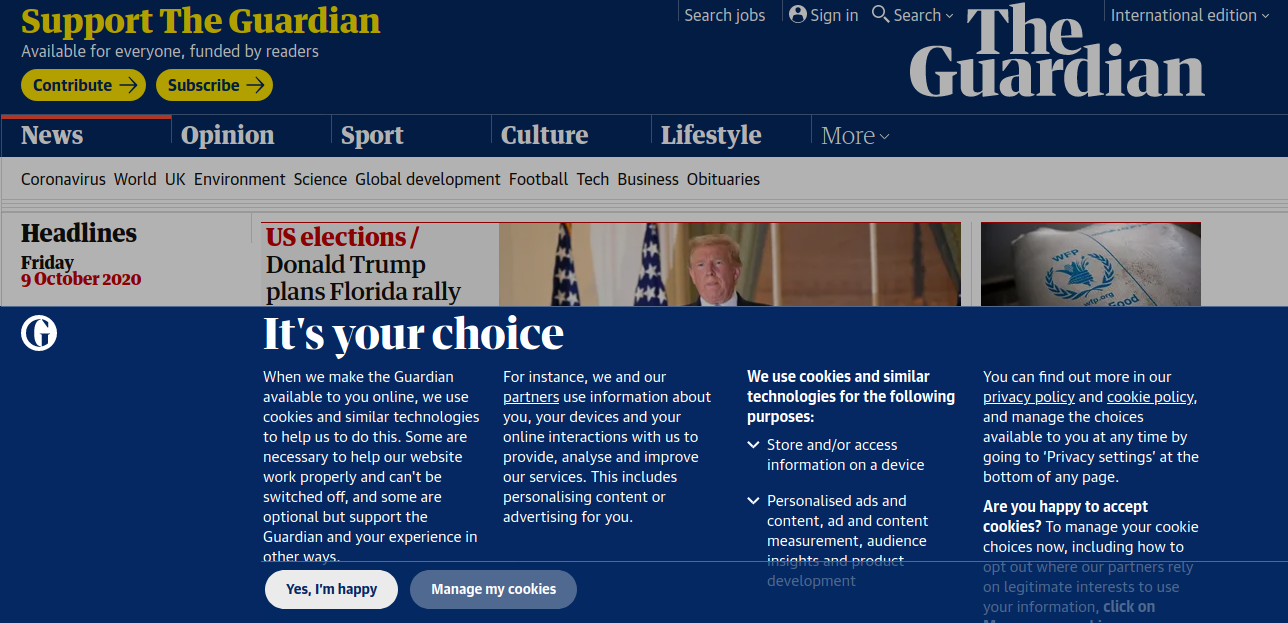
\includegraphics[width=\textwidth]{consent_form_guardian.png}
\caption{Consent form on The Guardian, a well-known British newspaper} \label{Figure 1}
\end{figure}

Overall, dark patterns are ubiquitous in the post-GDPR world \cite{ref9} and have challenged the rule of law by undermining key concepts such as consent \cite{ref10}. 

As such, when the goal is to purposefully trick users into giving away their data, and in so doing ridding themselves of their own right and concept of privacy, companies are engaging in a game of cat and mouse with regulators as to which one will be able to innovate over the other in the race for more market shares and better user leverage.

\section{Conclusions}
While the pros rightly outweighs the cons on paper and with regards to the topic of costs, the emergence of dark patterns is an issue that ought to be addressed. 

Indeed, while fear-mongering about compliance costs was used over the past few years to create a bulwark against GDPR, the main issue at hand is the emergence of dark patterns to circumvent the law and wrestle consent not from just EU citizens but everyone. 

As dark patterns muddy our concept of consent, privacy and trust, we ought to address how companies are gaming our senses and use our form-filling fatigue against us. A long battle is paved ahead of us if we wish for a world where the right of private property extend to our own personal data.

\section{Acknowledgments}
Thanks to the Université Côte d'Azur administration for creating a new class aimed at teaching proper scientific writing to the student corps.
%
%\section{References}
% ---- Bibliography ----
% BibTeX users should specify bibliography style 'splncs04'. References will then be sorted and formatted in the correct style.
\bibliographystyle{unsrt} %splncs04
%\renewcommand{\refname}{}
\bibliography{references}
%
\end{document}
